\section{Zooid}

\begin{frame}
  \vfill
  \begin{sticky}
  {\large
    \textbf{\underline{Zooid}}:
    A
    DSL
    for
    Certified
    Multiparty
    Computation\par
  }
  \end{sticky}
\end{frame}

\begin{frame}
  \frametitle{Zooid}
  {\color{gray}%
    /\phoneticZooidA, \phoneticZooidB, \phoneticZooidC\hspace{-.2cm}/}
  \vspace{.4cm}

  \emph{noun} %
  \only<1>{\textsc{zoology}}%
  \only<2->{\textsc{\sout{zoology}{\color{purple}computing}}}
  \vspace{.4cm}

  % \uncover<1>{an animal arising from another by budding or division, especially}
  each of the
  $\stackrel{\text{\normalsize%
      \uncover<2->{\color{purple}processes}}
  }{\text{%
      \only<1>{individuals}\only<2->{\sout{individuals}}}
  }$
  which make up a
  $\stackrel{\text{\normalsize%
      \uncover<2->{\color{purple}distributed system}}
  }{\text{%
      \only<1>{colonial organism}\only<2->{\sout{colonial organism}}}
  }$
  and typically have
  \only<1-2>{different forms and functions}%
  \only<3>{\textbf{\underline{different forms and functions}}}.
\end{frame}

\begin{frame}
  \frametitle{The Problem}

  Deadlocks are hard to avoid and debug in distributed systems.
  \vspace{.5cm}

  To address this, there are many tools for deadlock avoidance/detection.
  \vspace{1cm}

  But \emph{can we trust these tools}?
\end{frame}

\begin{frame}[fragile]
  \frametitle{Our Approach}
  \begin{picture}(0,0)
    {\put(300,65){
        \begin{tabular}{@{}c@{}}
          
\includegraphics[height=2.5cm]{figures/coq-logo.png}
          \\[-.5cm]
          {\tiny ``Le coq mécanisé'' by Lilia Anisimova}
        \end{tabular}
      }}
  \end{picture}

  A \redbf{certified} framework for verifying and implementing individual
  processes of a distributed system.
\end{frame}

\begin{frame}[fragile]
  \frametitle{Zooid Framework}

  \centering
  \begin{tikzpicture}
    [ global/.style={rounded rectangle, fill=purple!10, font=\scriptsize},
    proc/.style={rounded rectangle, fill=DarkRed!10, font=\scriptsize},
    code/.style={rounded rectangle, fill=DarkGreen!10, font=\scriptsize},
      zooid/.style={draw, thick, ellipse},
      proof/.style={rounded rectangle, fill=DarkBlue!10, font=\scriptsize},
      connector/.style={-{Stealth[scale=1.3]}, very thick, shorten >=3pt,shorten <= 3pt},
      semiauto/.style={{Stealth[scale=1.3]}-{Stealth[scale=1.3]}, very thick, shorten >=3pt,shorten <= 3pt, dotted}
    ]
    \node[global] (gt) {$\G$: global specification};
    \node[proc, right=1cm of gt] (proc) {\scriptsize$\zooid$: Zooid process.};
    \coordinate (mid) at ($(gt)!.5!(proc)$);
    \node[zooid, below=1cm of mid] (zooid) { Zooid };
    \node[proof, right=1.5cm of zooid] (pInG) { Proof that $\zooid$ behaves as $\p\in\G$ };

    \node[proof, below=1cm of zooid, xshift=-2cm] (WF) { Proof that $\G$ is well-formed};
    \node[code, below=1cm of zooid, xshift=2cm] (ocaml) { OCaml code for $\zooid$ };

    \draw[connector] (gt) -- (zooid);
    \draw[connector] (proc) -- (zooid);
    \draw[semiauto] (pInG) -- (zooid);
    \draw[connector] (zooid) -- (WF);
    \draw[connector] (zooid) -- (ocaml);
  \end{tikzpicture}

\end{frame}

\begin{frame}
  \vfill
  \begin{sticky}
  {\large
    Zooid:
    A
    DSL
    for
    Certified
    \textbf{\underline{Multiparty}}
    Computation\par
  }
  \end{sticky}
\end{frame}

\begin{frame}
  \frametitle{Multiparty Session Types in a Nutshell}
  \vskip.1cm
  \begin{center}
    \only<1>{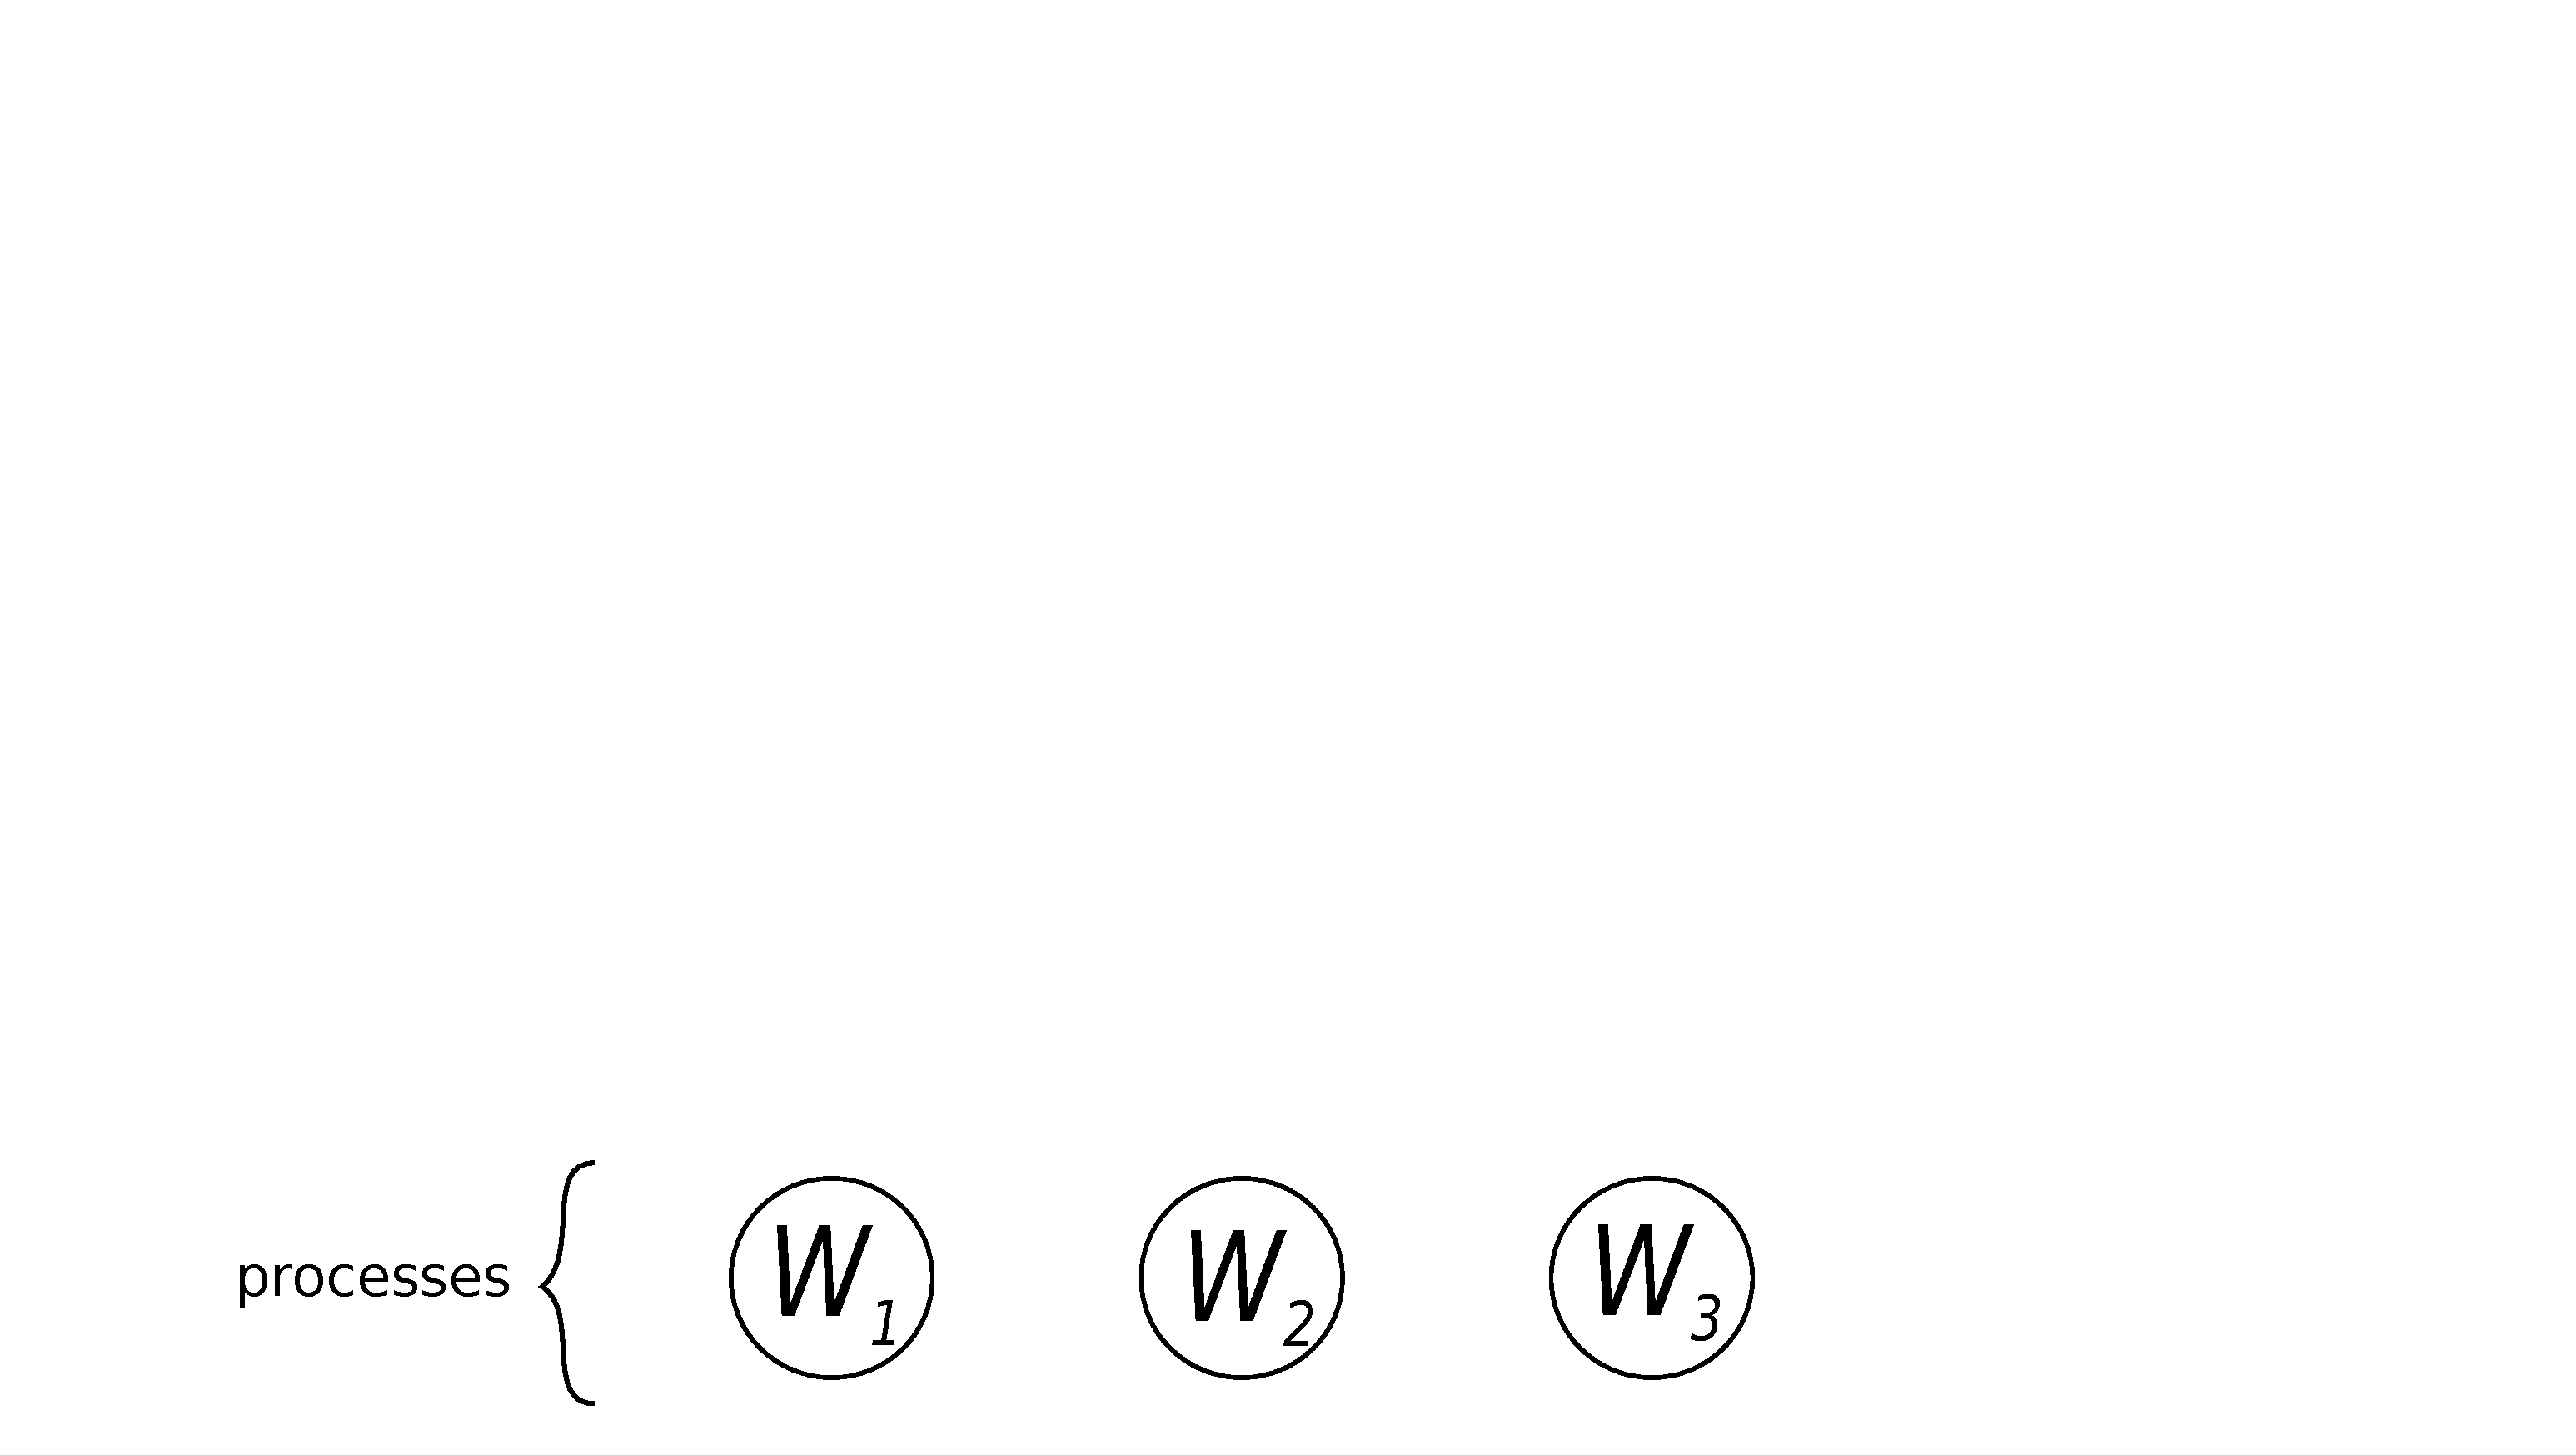
\includegraphics[width=.8\textwidth]{figures/MPST1.pdf}}%
    \only<2>{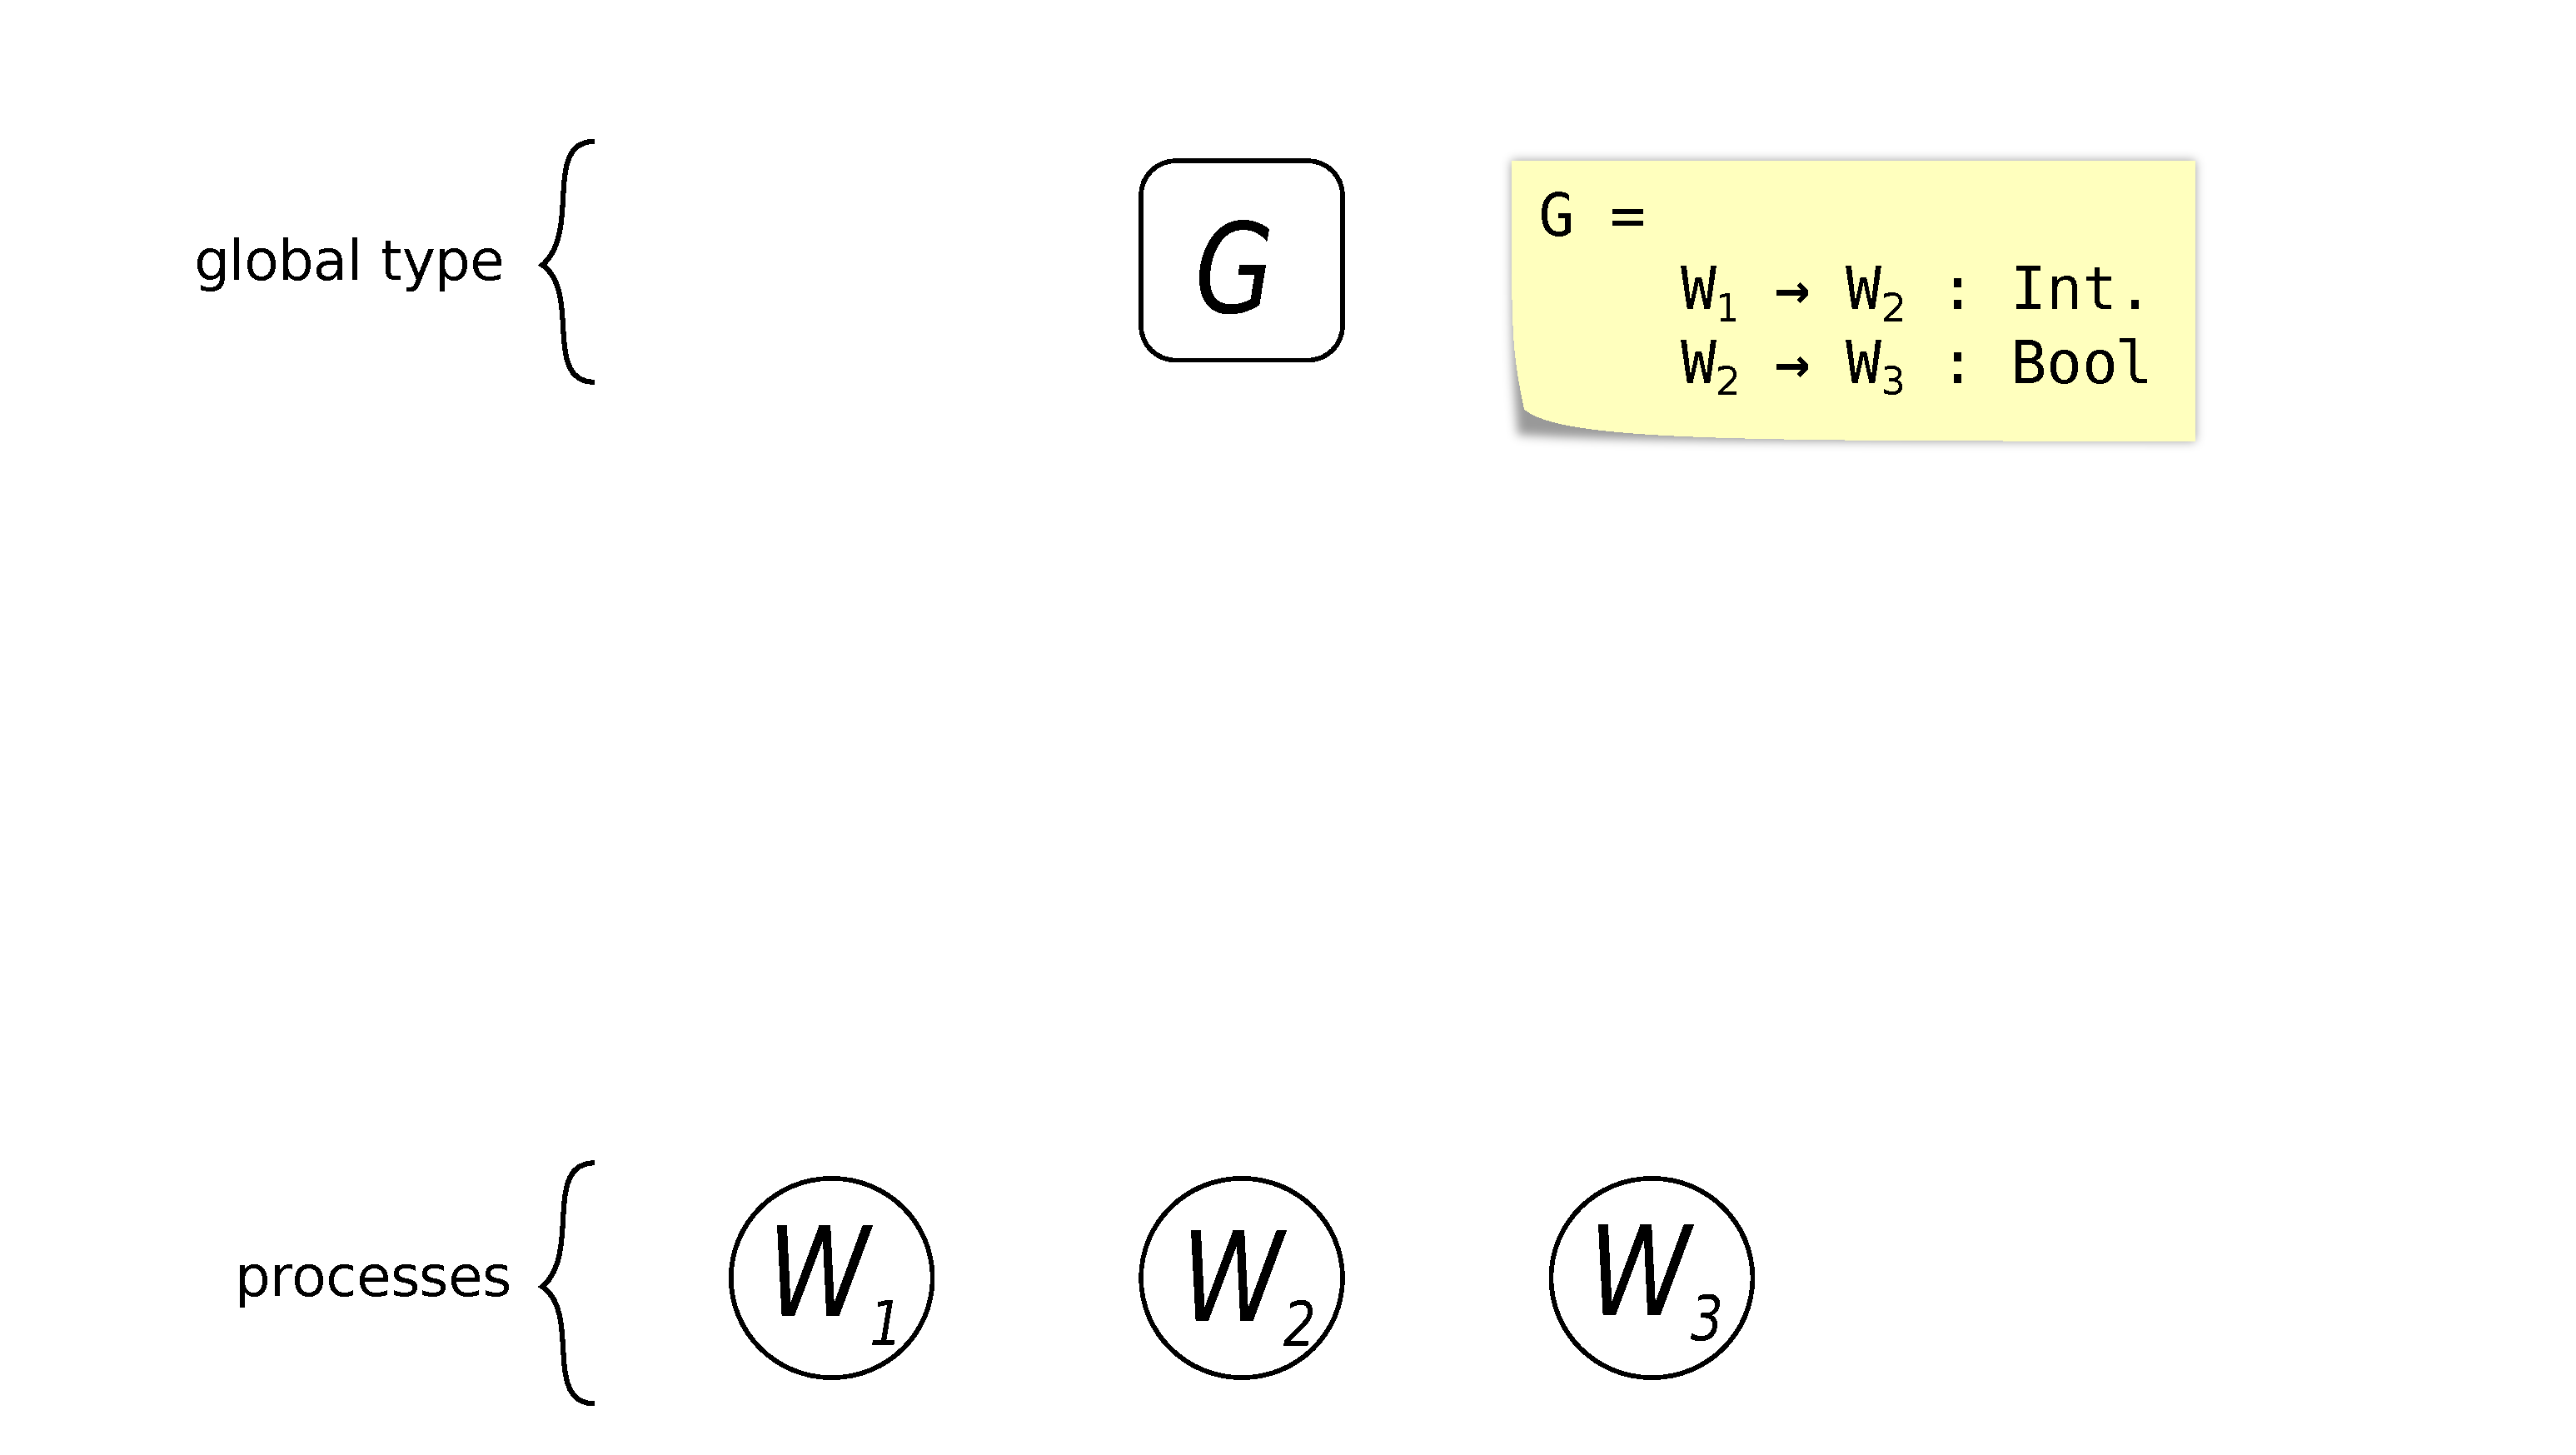
\includegraphics[width=.8\textwidth]{figures/MPST2.pdf}}%
    \only<3>{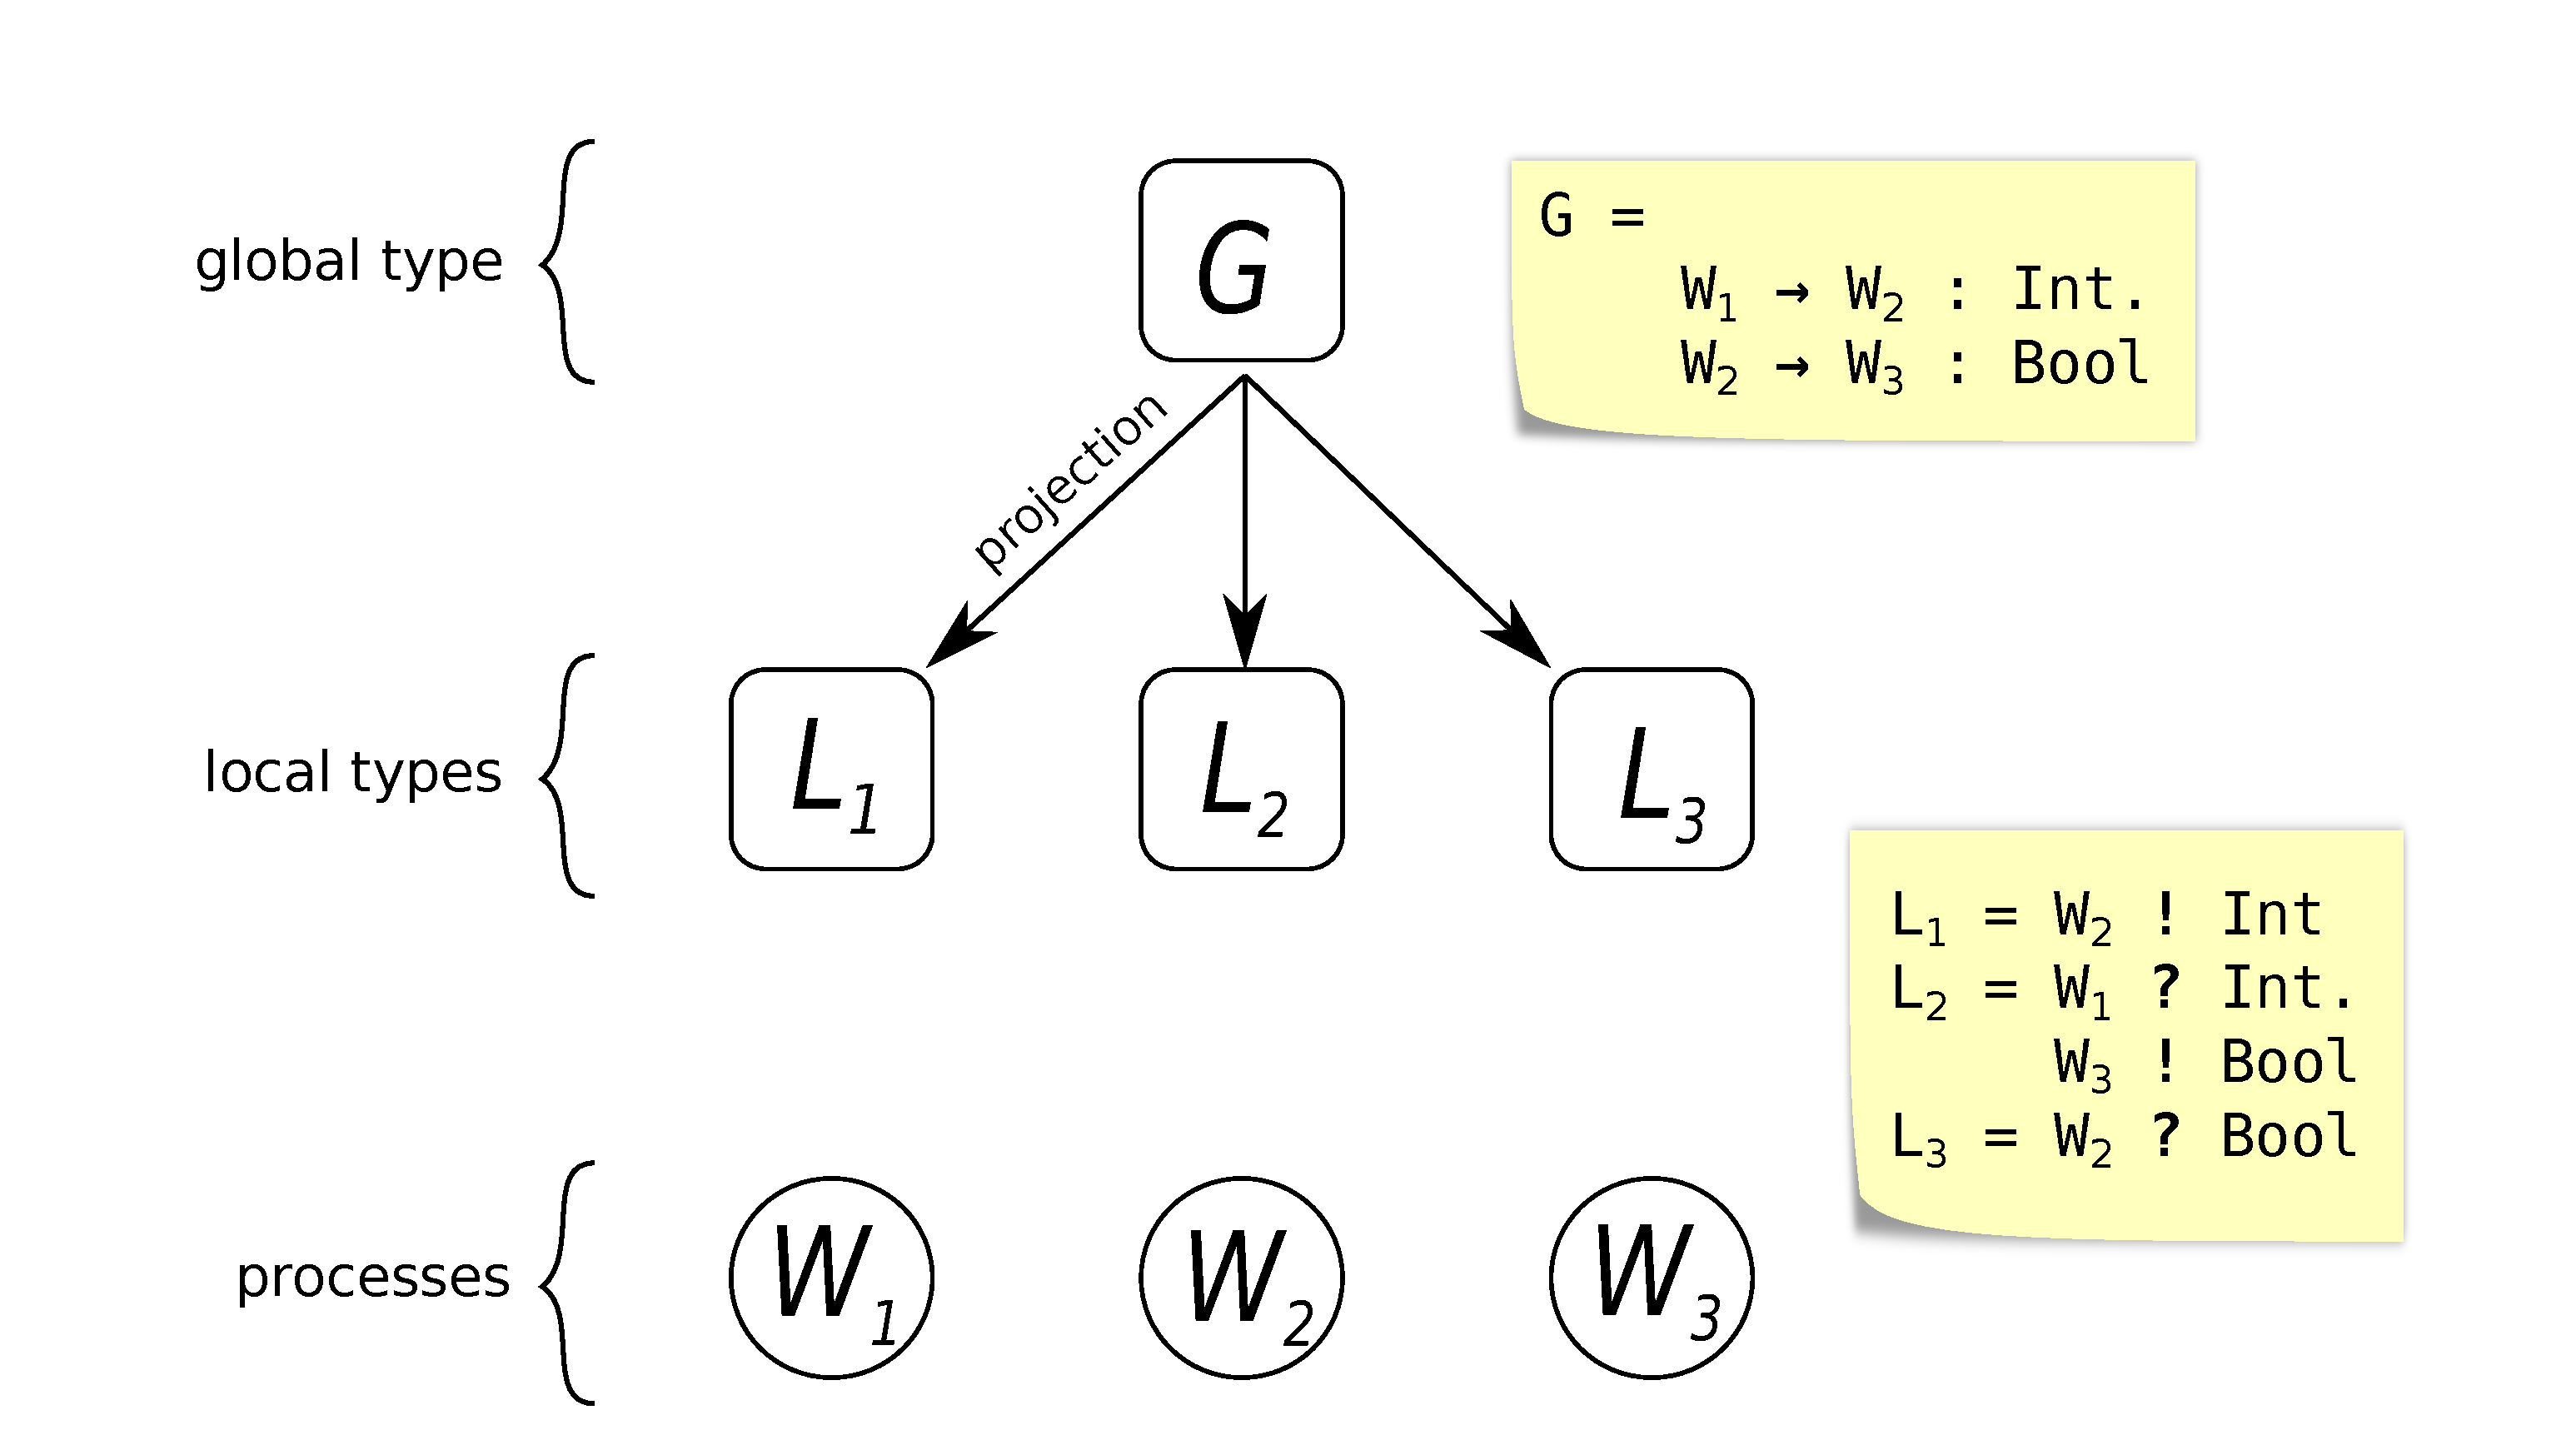
\includegraphics[width=.8\textwidth]{figures/MPST3.pdf}}%
    \only<4>{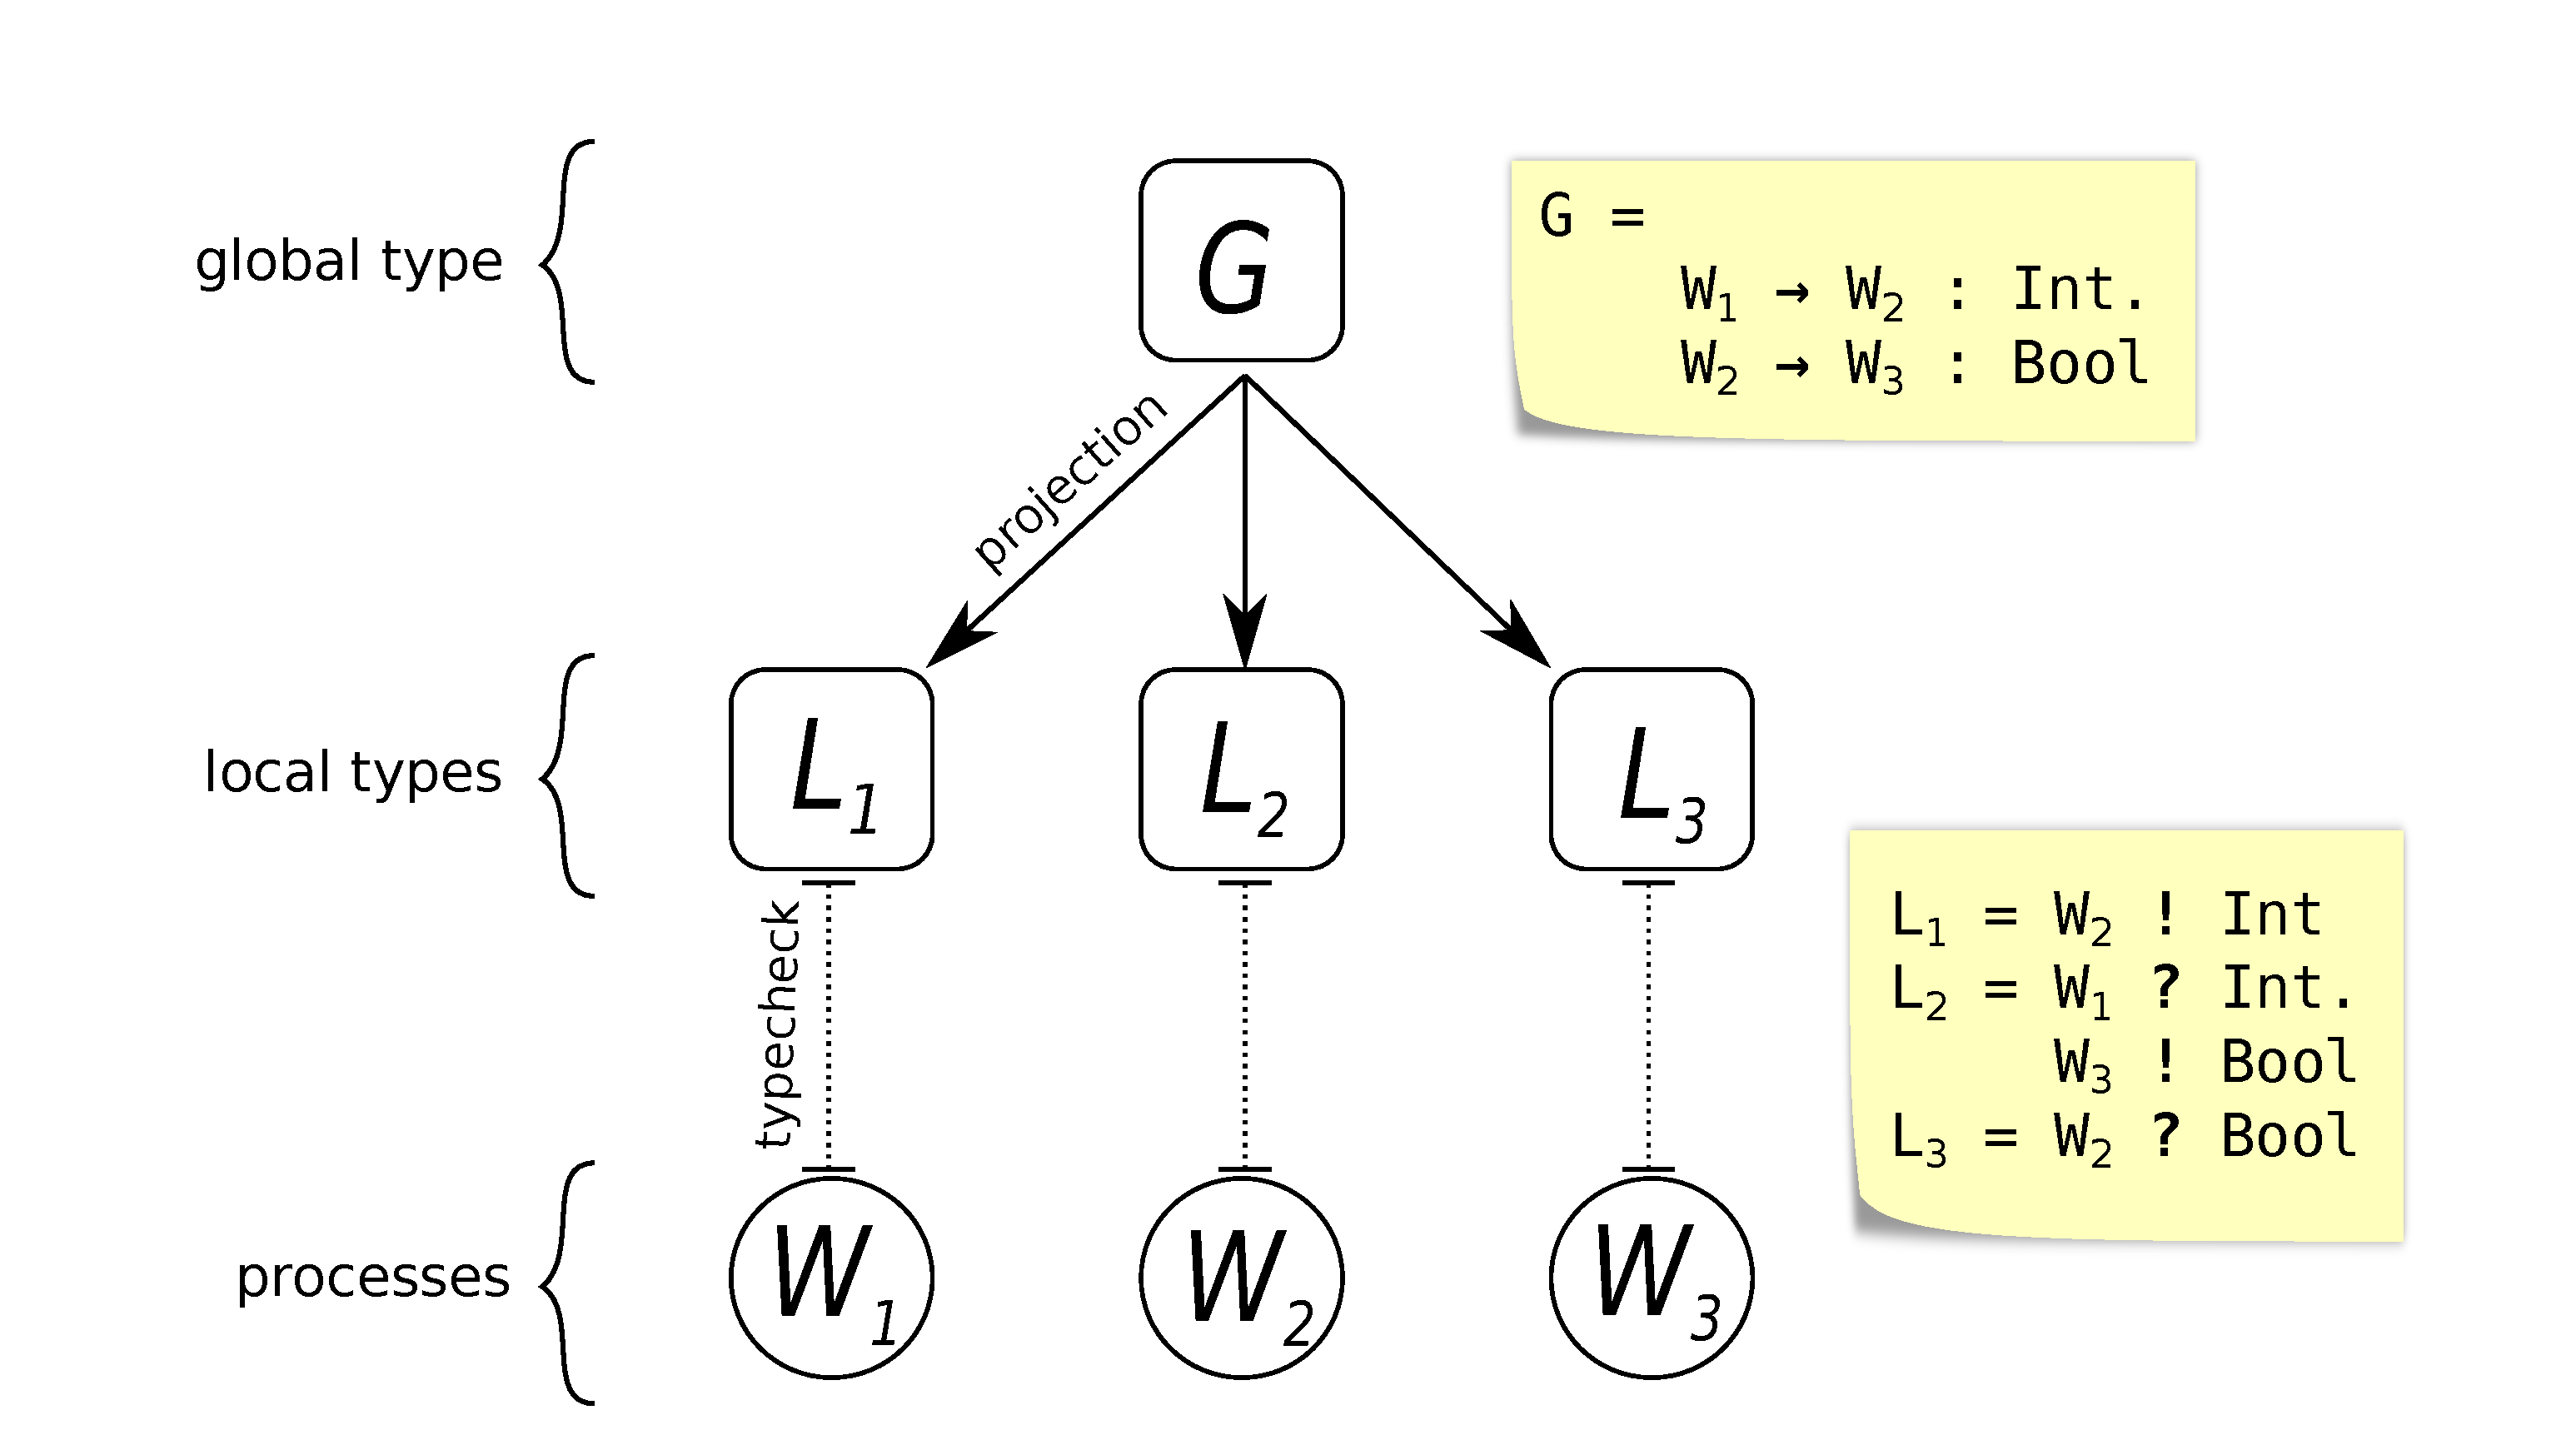
\includegraphics[width=.8\textwidth]{figures/MPST4.pdf}}%
    \only<5>{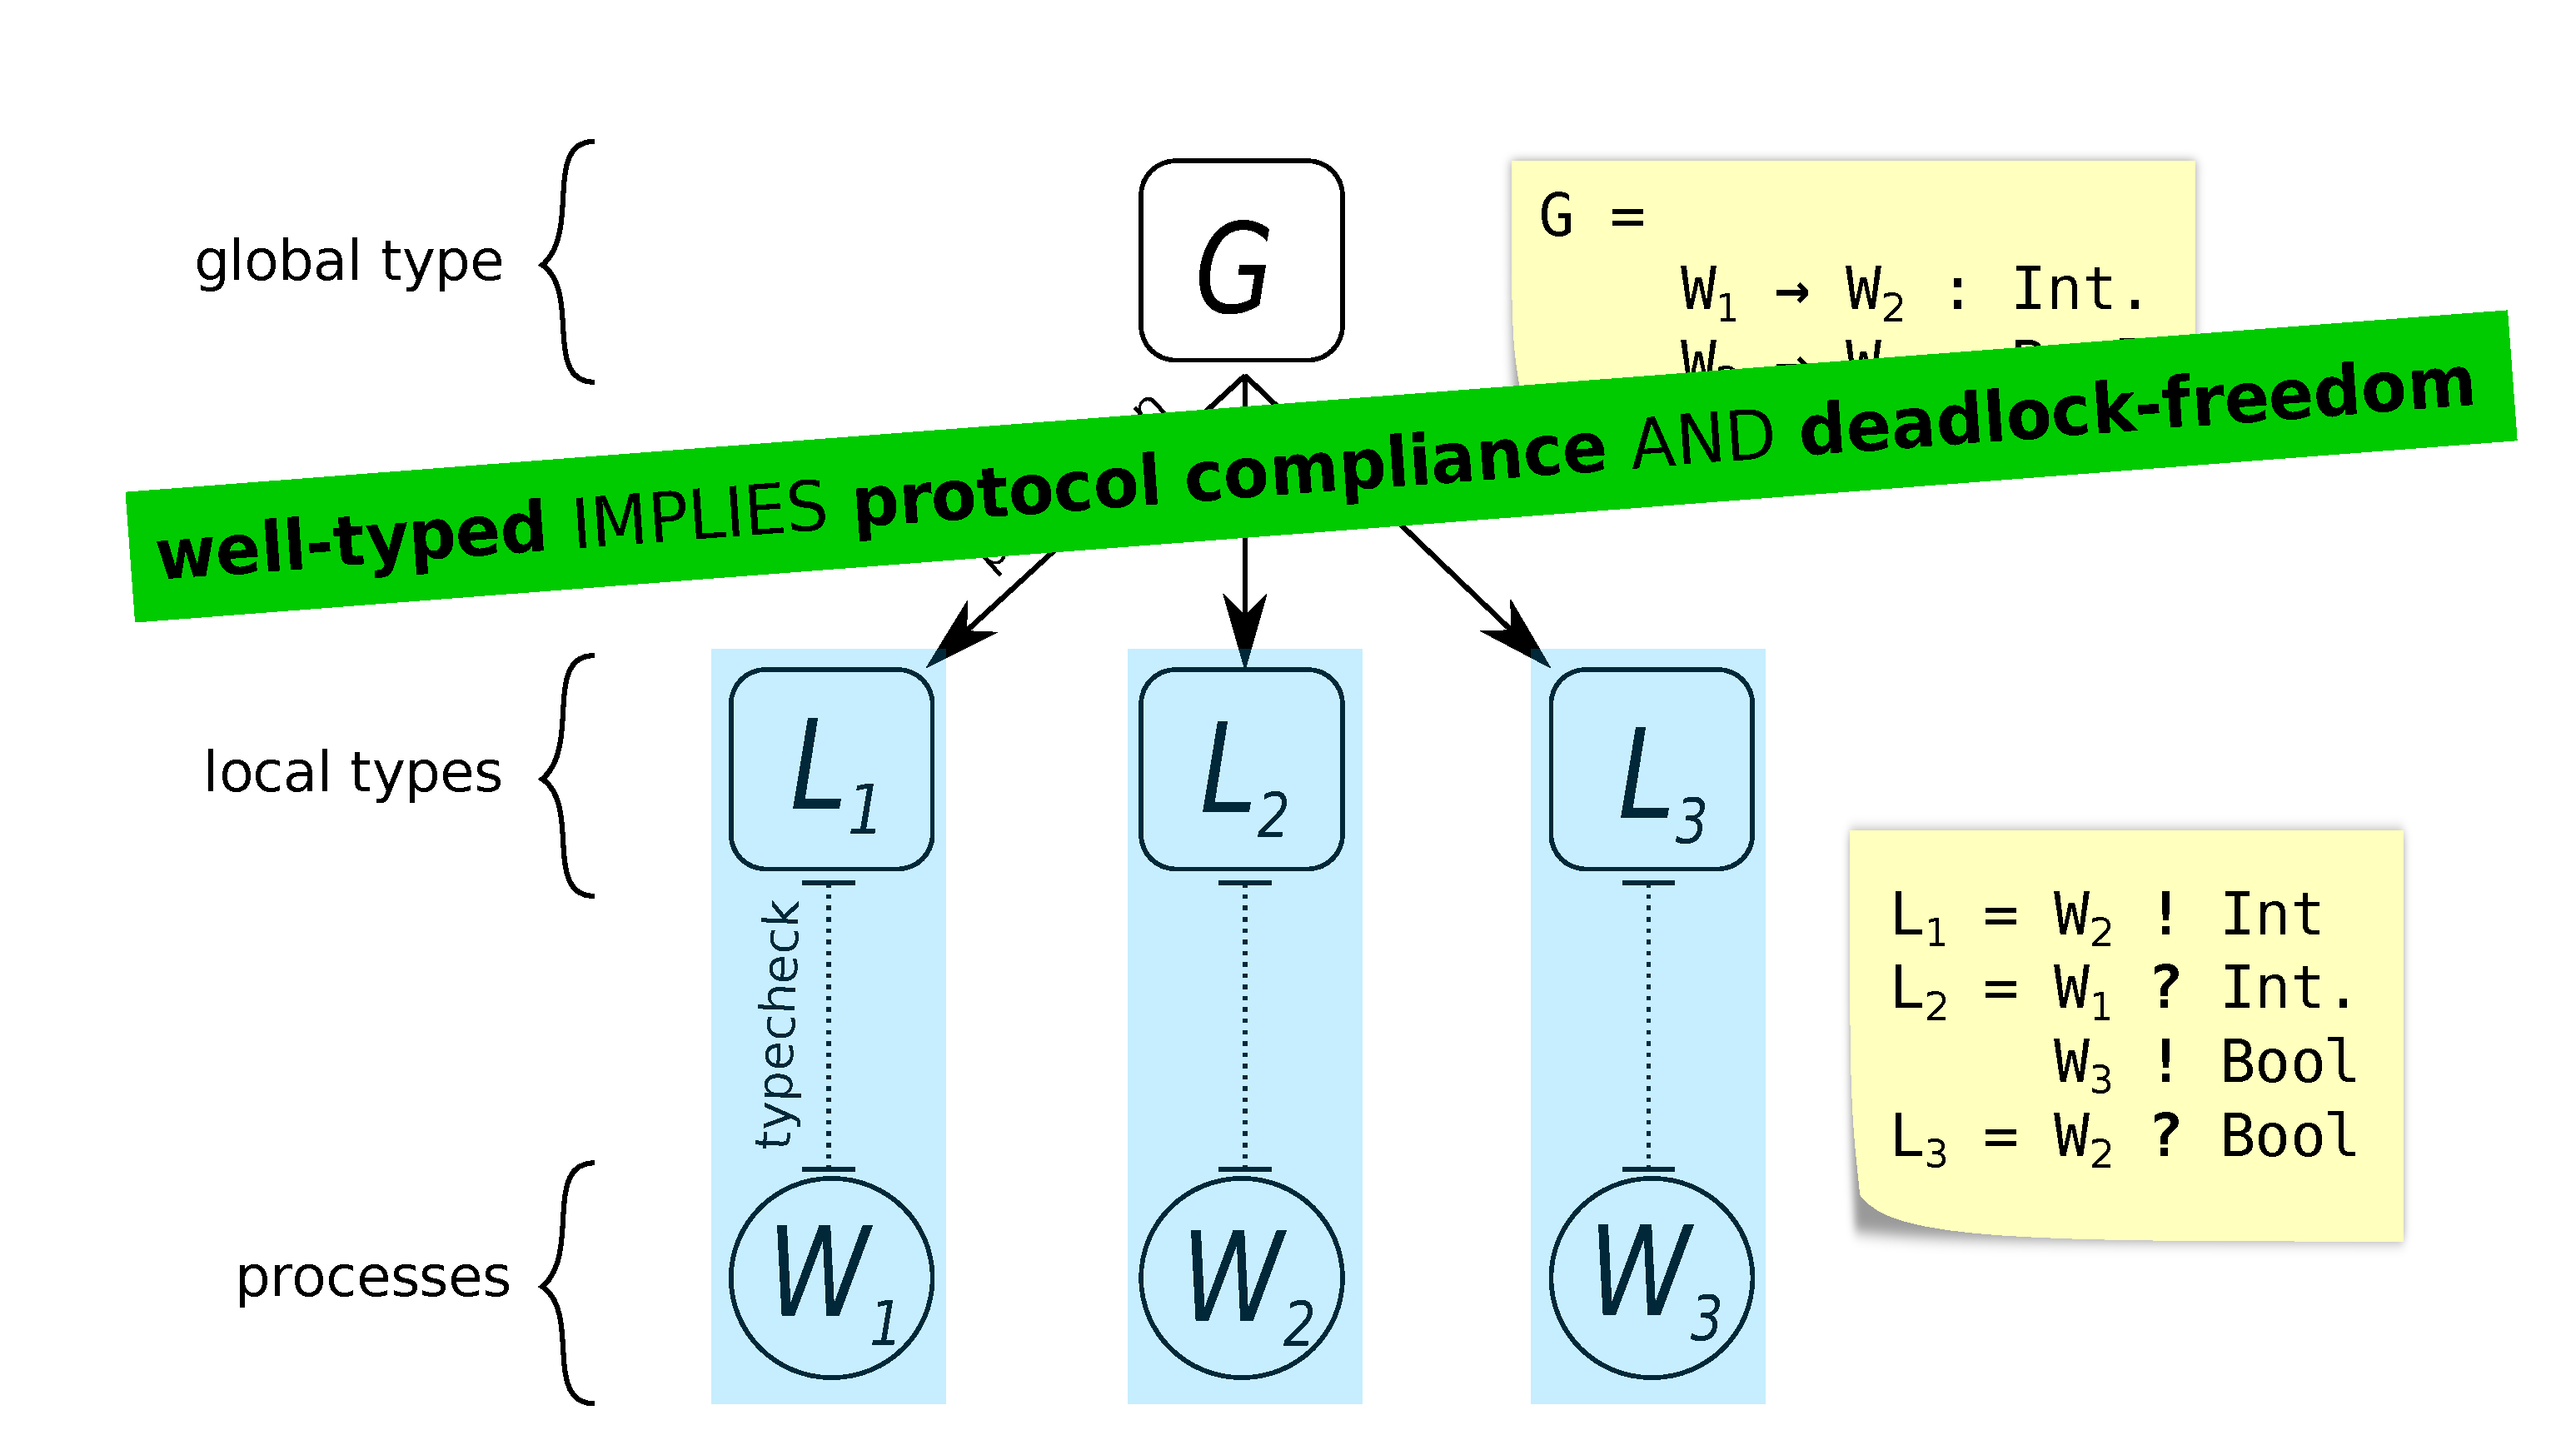
\includegraphics[width=.8\textwidth]{figures/MPST5.pdf}}
  \end{center}
\end{frame}


\begin{frame}
  \vfill
  \begin{sticky}
  {\large
    Zooid:
    A
    DSL
    for
    \textbf{\underline{Certified}}
    Multiparty
    Computation\par
  }
  \end{sticky}
\end{frame}

\pgfdeclarelayer{background}
\pgfsetlayers{background,main}
\begin{frame}<0>[noframenumbering]
  \frametitle{Overview}

  \centering
  \begin{tikzpicture}[commutative diagrams/every diagram]
    \begin{pgfonlayer}{background}
      \fill[rounded corners, yellow!20!white] (-0.8,0.5) rectangle (7.5,-3.5);
    \end{pgfonlayer}
    
    \node(G0)at (0,0) {$\G$};
    \node(G1)at (3,0) {$\coG$};
    \node(G2)at (6,0) {\small{global trace}};
    \node(L0)at (0,-1.5) {$\lT$};
    \node(L1)at (3,-1.5) {$\colT$};
    \node(L2)at (6,-1.5) {\small{local trace}};
    \node(M1)at (1.5,-0.75) {\small{\textcolor{orange}{(M.1)}}};
    \node(M2)at (4.5,-0.75) {\small{\textcolor{orange}{(M.2)}}};
    \node(P0)at (0,-3) {$\proc$};
    \node(P2)at (6,-3) {\small{process trace}};
    \node(M3)at (3.3,-2.25) {\small{\textcolor{orange}{(M.3)}}};
    \node(OC)at (0,-5) {\small{OCaml code}};
    \node(ZZ)at (3.5,-5) {\bf \dslName};
     
     \path[commutative diagrams/.cd,every arrow,font=\scriptsize]
     (G0) edge node[above] {$\Re$} (G1)
     (G1) edge node[above] {LTS} (G2)
     (L0) edge node[above] {$\Re$} (L1)
     (L1) edge node[above] {LTS} (L2)
     (G0) edge node[right] {$\upharpoonright$} (L0)
     (G1) edge node[right] {$\upharpoonright^{\textsf{c}}$} (L1)
     (G2) edge[<->] node[right] {$=$} (L2)
     (L0) edge node[right] {$\ofLt$} (P0)
     (P0) edge node[above, xshift=-.5cm] {LTS} (P2)
     (P2) edge node[right] {erase} (L2)
     (P0) edge node[left] {extraction} (OC)
     (P0) edge[<->] node[right,xshift=.1cm] {DSL layer} (ZZ)
     ;
     \path[dashed, red, commutative diagrams/.cd, font=\scriptsize]
     (L0) edge[bend left=40] node[below left,yshift=.4cm, xshift=-.2cm]
       {Well typed!} (ZZ)
     (P2) edge[] node[below right] {Certified semantics!} (ZZ)
     (OC) edge[] node[above] {Extractable!} (ZZ)
     ;
  \end{tikzpicture}

\end{frame}


\begin{frame}[fragile]
  \frametitle{Mechanising Global/Local Types}
  Inductive or coinductive representations?

  \[
    \G \Coloneqq
    \gend
    \SEP \msgi{\p}{\q}{\ell}{\tS}{\G}
    \SEP \gX
    \SEP \grec{\gX}{\G}
  \]
  \[
    \coG \Coloneqq \cogend \SEP
    \comsgni \p\q \ell {\tS} {\coG}
    %\SEP \comsgsi  \p\q {\ell_j} \ell {\tS} {\coG}
  \]
\end{frame}

\begin{frame}[fragile]
  \frametitle{Syntactic Global Types}
  \[
    \G \Coloneqq
    \gend
    \SEP \msgi{\p}{\q}{\ell}{\tS}{\G}
    \SEP \gX
    \SEP \grec{\gX}{\G}
  \]
  \vfill
  \begin{columns}
    \begin{column}[t]{.49\textwidth}
      \begin{greenbox}{}
        \small
        We can:
        \begin{itemize}% [leftmargin=*]
        \item[$\itm$] \emph{decide} properties on $\G$
        \item[$\itm$] \emph{compute} functions on $\G$
        \end{itemize}
      \end{greenbox}
    \end{column}
    \begin{column}[t]{.49\textwidth}
        \begin{redbox}
          \small
          We require:
          \begin{itemize}%[leftmargin=*]
          \item[$\itm$] $\grec{\gX}{\G} \equiv [\grec{\gX}{\G}/\gX]\G$
          \item[$\itm$] carrying many properties around (e.g. guardedness)
          \end{itemize}
        \end{redbox}
      \end{column}
    \end{columns}
\end{frame}

\begin{frame}[fragile]
  \frametitle{Coinductive Global Trees}
  \[
    \coG \Coloneqq \cogend \SEP
    \comsgni \p\q \ell {\tS} {\coG}
    % \SEP \comsgsi  \p\q {\ell_j} \ell {\tS} {\coG}
  \]
  \vfill
  \begin{columns}
    \begin{column}[t]{.49\textwidth}
      \begin{greenbox}{}
        \small
        \begin{itemize}%[leftmargin=*]
        \item[$\itm$] Coq guarantees guardedness and closedness.
        \item[$\itm$] Bisimilarity is easier to deal with than
          $\grec{\gX}{\G} \equiv [\grec{\gX}{\G}/\gX]\G$.
        \end{itemize}
      \end{greenbox}
    \end{column}
    \begin{column}[t]{.49\textwidth}
      \begin{redbox}
        \small
        \begin{itemize}%[leftmargin=*]
        \item[$\itm$] We can only inspect a finite part of $\coG$
        \item[$\itm$] We can only decide properties on prefixes of $\coG$
        \end{itemize}
      \end{redbox}
    \end{column}
  \end{columns}
\end{frame}

\begin{frame}[fragile]
  \frametitle{Unravelling}
  $\G \leadsto [\grec{\gX}{\G}/\gX]\G \leadsto [[\grec{\gX}{\G}/\gX]\G/\gX]\G
  \leadsto \cdots \leadsto \coG$

  \vspace{1cm}
  \begin{itemize}
  \item[\itm] We use a form of {\color{blue}\textbf{coinductive reflection}}:
    \begin{itemize}
      \item properties that are
        decided on $\G$ are guaranteed on $\coG$.
      \end{itemize}
  \item[\itm] $\G$ is checked for guardedness and closedness once.
  \item[\itm] Guardedness and closedness are straightforwardly true for $\coG$.
  \end{itemize}
\end{frame}

\begin{frame}
  \frametitle{Mechanising Projection}
  \begin{center}
  \begin{minipage}{.35\columnwidth}
  \begin{sticky}
  \begin{tikzpicture}[commutative diagrams/every diagram]
    % \begin{pgfonlayer}{background}
    %   \fill[rounded corners, yellow!20!white] (-0.8,0.5) rectangle (4,-2);
    % \end{pgfonlayer}
    
    \node(G0)at (0,0) {$\G$};
    \node(G1)at (3,0) {$\coG$};
    \node(L0)at (0,-1.5) {$\lT$};
    \node(L1)at (3,-1.5) {$\colT$};
     
     \path[commutative diagrams/.cd,every arrow,font=\scriptsize]
     (G0) edge node[above] {$\Re$} (G1)
     (L0) edge node[above] {$\Re$} (L1)
     (G0) edge node[right] {$\upharpoonright$} (L0)
     (G1) edge node[right] {$\upharpoonright^{\textsf{c}}$} (L1)
     ;
  \end{tikzpicture}
  \end{sticky}
  \end{minipage}
  \end{center}
  \begin{itemize}
    \item[\itm] $\Re$ is the unravelling relation.
    \item[\itm]
      \only<1>{{$\upharpoonright$ is a \redbf{function}, but
          $\upharpoonright^{\textsf{c}}$ is a \redbf{relation}}}%
      \only<2>{\emph{$\upharpoonright$ is a \redbf{function}, but
          $\upharpoonright^{\textsf{c}}$ is a \redbf{relation}}}.
  \end{itemize}
\end{frame}

\begin{frame}
  \frametitle{Coinductive Projection}
  \uncover<2->{So why not a corecursive function?}
  \vspace{1cm}
  \only<1-2>{
    \[
      \mprset{fraction={===}}
      \inferrule*[lab=\rulename{co-proj-send-1}]
      {
        \pr=\p \\
        \forall i\in I. \coproj {\pr} {\coG_{\dcog i}} {\colT_{\dcol i}} 
      }
      {
        \coproj{%
          \pr
        }{%
          \comsgni \p\q \ell {\tS} {\coG}
        }{%
          \colsend \q \ell {\tS} {\colT}
        }
      }
    \]
  }\only<3->{
  \[
    \inferrule*[lab=\rulename{co-proj-cont}]
    {
      \pr\neq\p \quad
      \pr\neq\q \\\\
      \forall i\in I. \coproj {\pr}{\coG_{\dcog i}}{\colT_{\dcol i}} \quad
      \only<3>{%
        \forall i,j\in I. \colT_{\dcol i}=\colT_{\dcol j}
      }\only<4>{%
        \mathcolorbox{red!20}{\forall i,j\in I. \colT_{\dcol i}=\colT_{\dcol j}}
      } \quad
      \only<3>{%
        \forall i\in I. \partof \pr {\coG_{\dcog i}}
      }\only<4>{%
      \mathcolorbox{yellow!20}{\forall i\in I. \partof \pr {\coG_{\dcog i}}}
      }
    }
    {
      \coproj {\pr} { \comsgni \p\q \ell {\tS} {\coG} } {%
        \only<3>{\colT_{\dcol 1}}\only<4>{\mathcolorbox{yellow!20}{\colT_{\dcol 1}}}
      }
    }
  \]
}
% \uncover<4>{
%   \begin{itemize}
%     \item[\itm] \hlfancy{red!20}{Cannot} decide if two coinductive local types
%       are equal; and
%     \item[\itm] \hlfancy{yellow!20}{Difficult} to guarantee guardedness (and
%       requires mixing induction and coinduction).
%   \end{itemize}
% }
\end{frame}

\begin{frame}
  \frametitle{Semantics}

  \centering
  \begin{minipage}{.5\columnwidth}
    \begin{sticky}
  \begin{tikzpicture}[commutative diagrams/every diagram]
    \node(G1)at (3,0) {$\coG$};
    \node(G2)at (6,0) {\small{global trace}};
    \node(L1)at (3,-1.5) {$\colT$};
    \node(L2)at (6,-1.5) {\small{local trace}};
     
     \path[commutative diagrams/.cd,every arrow,font=\scriptsize]
     (G1) edge node[above] {LTS} (G2)
     (L1) edge node[above] {LTS} (L2)
     (G1) edge node[right] {$\upharpoonright^{\textsf{c}}$} (L1)
     (G2) edge[<->] node[right] {$=$} (L2)
     ;
  \end{tikzpicture}
  \end{sticky}
  \end{minipage}
\end{frame}

\begin{frame}[fragile]
  \frametitle{Trace Equivalence}
  \begin{minted}{coq}
    Theorem IndTraceEquiv g (WF : well_formed g)
      : forall trace,
          gty_accepts trace g <->
          lty_accepts trace (project_env WF).
  \end{minted}
\end{frame}

\begin{frame}
  \vfill
  \begin{sticky}
  {\large
    Zooid:
    A
    \textbf{\underline{DSL}}
    for
    Certified
    Multiparty
    Computation\par
  }
  \end{sticky}
\end{frame}

\begin{frame}[fragile]
  \frametitle{Core Processes}
  \small
  \begin{minted}{coq}
Inductive Proc :=
| Finish | Jump (v : nat) | Loop of Proc
| Recv (p : role) of Alts
| Send (p : role) T (l : lbl) : coq_ty T -> Proc -> Proc
(* external actions *)
| InteractWithEnv Tw Tr
  : (coq_ty Tw -> coq_ty Tr) ->
      coq_ty Tw -> (coq_ty Tr -> Proc) -> Proc
with Alts :=
| A_sing {T} (l : lbl) : (coq_ty T -> Proc) -> Alts
| A_cons {T} (l : lbl) : (coq_ty T -> Proc) -> Alts -> Alts.
  \end{minted}
\end{frame}

\begin{frame}[fragile]
  \frametitle{Zooid -- From Mechanised Metatheory to Impl.}

  \begin{itemize}
    \item Zooid constructs are \textbf{smart constructors} that package:
      \begin{itemize}
        \item a core process;
        \item a local type; and
        \item a proof that the process is \textbf{well-typed} with respect to
          the local type
      \end{itemize}
  \end{itemize}
  \begin{sticky}%
  {\small%
    \vspace{-.8cm}
  \begin{minted}{coq}
  Definition Zooid L := { P : Proc  | of_lt P L }.

  Definition wt_send p l T (pl : coq_ty T) L (P : Zooid L)
  : Zooid (l_msg l_send p [::(l, (T, L))]) := ...
  \end{minted}
  }
  \end{sticky}
  
\end{frame}

\begin{frame}[fragile]
  \frametitle{Connecting Zooid with Global Types (I)}
  Given $\G \upharpoonright \p$ and a term $Z : \mathsf{Zooid}\hspace{.2cm}\lT$:
  \begin{itemize}
    \item In most cases an automatic check can show syntactic equality: $\G
      \upharpoonright \p = \lT$.
    \item Some cases may require straightforward proofs that unrolling $\lT$ and
$\G \upharpoonright \p$ yields the same local type.
  \end{itemize}
\end{frame}

\begin{frame}[fragile]
  \frametitle{Connecting Zooid with Global Types (and II)}
  We prove that if a zooid term is well-typed with respect to $\G \upharpoonright\p$,
  then its trace is accepted by $\G$.

  \begin{sticky}
    \small
    \vspace{-.9cm}
  \begin{minted}{coq}
Theorem process_traces_are_global_types G p iPe P :
  eproject simple_merge G == Some iPe -> of_lt_unr p P iPe ->
  forall PTRACE, p_accepts p PTRACE P ->
    exists TRACE,
      gty_accepts TRACE G /\ subtrace p (erase PTRACE) TRACE.
  \end{minted}
  \end{sticky}
\end{frame}

\begin{frame}[fragile, noframenumbering]
  \frametitle{Connecting Zooid with Global Types (and II)}
  We prove that if a zooid term is well-typed with respect to $\G \upharpoonright\p$,
  then its trace is accepted by $\G$.

    \tikzset{
      ncbar angle/.initial=90,
      ncbar/.style={
        to path=(\tikztostart)
        -- ($(\tikztostart)!#1!\pgfkeysvalueof{/tikz/ncbar angle}:(\tikztotarget)$)
        -- ($(\tikztotarget)!($(\tikztostart)!#1!\pgfkeysvalueof{/tikz/ncbar angle}:(\tikztotarget)$)!\pgfkeysvalueof{/tikz/ncbar angle}:(\tikztostart)$)
        -- (\tikztotarget)
      },
      %      ncbar/.default=0.5cm,
            ncbar/.default=0.3cm,
    }
    \tikzset{square left brace/.style={ncbar=0.1cm}}

    \begin{sticky}
    \begin{tikzpicture}
      \node[text=\colorgt] (a1) {\small $\coG_1$ };
      \node[text=\colorgt  , right = .35cm of a1] (a2) {\small $\coG_2$ };
      \node[text=\colorgt  , right = .35cm of a2] (a3) {\small $\coG_3$ };
%      \node[text=\colorgt  , right = .35cm of a3] (a4) {\small $\coG_4$ };
      \node[                 right = .35cm of a3] (d1) {\small $\cdots$ };
      \node[text=\colorgt  , right = .35cm of d1] (a5) {\small $\coG_5$ };
      \node[text=\colorgt  , right = .35cm of a5] (a6) {\small $\coG_6$ };
%      \node[text=\colorgt  , right = .35cm of a6] (a7) {\small $\coG_7$ };
      \node[                 right = .35cm of a6] (d2) {\small $\cdots$ };

      \path[draw, ->] (a1) -- (a2) node[midway, above, text = \colorgt] {\footnotesize $a_1$ };
      \path[draw, ->] (a2) -- (a3) node[midway, above, text = \colorproc] (g2) {\footnotesize $a_2$ };
%      \path[draw, ->] (a3) -- (a4) node[midway, above, text = \colorgt] {\footnotesize $a_3$ };
      \path[draw, ->] (a3) -- (d1) node[midway, above, text = \colorgt] { };
      \path[draw, ->] (d1) -- (a5) node[midway, above, text = \colorgt] {\footnotesize $a_4$ };
      \path[draw, ->] (a5) -- (a6) node[midway, above, text = \colorproc] (g6) {\footnotesize $a_5$ };
%      \path[draw, ->] (a6) -- (a7) node[midway, above, text = \colorgt] {\footnotesize $a_6$ };
      \path[draw, ->] (a6) -- (d2) node[midway, above, text = \colorgt] { };

      \node[text=\colorproc, above = .5cm of a1] (a2') {\small $\proc_1$ };
      \node[text=\colorproc, right = 1.0cm of a2'] (a5') {\small $\proc_2$ };
      \node[text=\colorproc, right = 1.0cm of a5'] (a6') {\small $\proc_3$ };
      \node[                 right = 1.0cm of a6'] (d2') {\small $\cdots$ };
      \path[draw, ->] (a2') -- (a5') node[above, midway, text = \colorproc] (p2) {\footnotesize $a_2$};
      \path[draw, ->] (a5') -- (a6') node[above, midway, text = \colorproc] (p6) {\footnotesize $a_5$};
      \path[draw, ->] (a6') -- (d2');

      \path[draw, thick, dotted, -, red] (g2) -- (p2);
      \path[draw, thick, dotted, -, red] (g6) -- (p6);


      \draw ($(a2')-(.5cm,.2cm)$) to [square left brace] ($(a2')+(-.5cm, .2cm)$)
       node[text=\colorproc, left, yshift=-.2cm, xshift=-.1cm] {$\forall t_\p$} ;

      \draw ($(a1)-(.5cm,.2cm)$) to [square left brace] ($(a1)+(-.5cm, .2cm)$)
       node[text=\colorgt, left, yshift=-.2cm, xshift=-.2cm] (t) {$\exists t$} ;

      % \node[draw, rectangle, above = 1cm of t] {If $\expr$ Forall $t_\p$ accepted by $\expr$, there exists a trace $t$};
    \end{tikzpicture}
    \end{sticky}
\end{frame}

\begin{frame}[fragile]
  \frametitle{Code Extraction}
  \begin{sticky}
    \small
    \vspace{-.8cm}
    \begin{minted}{coq}
Module ProcExtraction (MP : ProcessMonad).
  Fixpoint extract_proc (d : nat) (p : Proc) : MP.t unit :=
    match p with
    | Send p T l v k =>
      MP.bind (MP.send p l v) (fun=>extract_proc d k)
    | ...
    end.
End ProcExtraction.
    \end{minted}
\end{sticky}
  
\end{frame}

\begin{frame}
  \frametitle{Wrapping Up}

  \centering
  \begin{tikzpicture}[commutative diagrams/every diagram]
    \begin{pgfonlayer}{background}
      \fill[rounded corners, yellow!20!white] (-0.8,0.5) rectangle (7.5,-3.5);
    \end{pgfonlayer}
    
    \node(G0)at (0,0) {$\G$};
    \node(G1)at (3,0) {$\coG$};
    \node(G2)at (6,0) {\small{global trace}};
    \node(L0)at (0,-1.5) {$\lT$};
    \node(L1)at (3,-1.5) {$\colT$};
    \node(L2)at (6,-1.5) {\small{local trace}};
    \node(M1)at (1.5,-0.75) {\small{\textcolor{orange}{(M.1)}}};
    \node(M2)at (4.5,-0.75) {\small{\textcolor{orange}{(M.2)}}};
    \node(P0)at (0,-3) {$\proc$};
    \node(P2)at (6,-3) {\small{process trace}};
    \node(M3)at (3.3,-2.25) {\small{\textcolor{orange}{(M.3)}}};
    \node(OC)at (0,-5) {\small{OCaml code}};
    \node(ZZ)at (3.5,-5) {\bf \dslName};
     
     \path[commutative diagrams/.cd,every arrow,font=\scriptsize]
     (G0) edge node[above] {$\Re$} (G1)
     (G1) edge node[above] {LTS} (G2)
     (L0) edge node[above] {$\Re$} (L1)
     (L1) edge node[above] {LTS} (L2)
     (G0) edge node[right] {$\upharpoonright$} (L0)
     (G1) edge node[right] {$\upharpoonright^{\textsf{c}}$} (L1)
     (G2) edge[<->] node[right] {$=$} (L2)
     (L0) edge node[right] {$\ofLt$} (P0)
     (P0) edge node[above, xshift=-.5cm] {LTS} (P2)
     (P2) edge node[right] {erase} (L2)
     (P0) edge node[left] {extraction} (OC)
     (P0) edge[<->] node[right,xshift=.1cm] {DSL layer} (ZZ)
     ;
     \path[dashed, red, commutative diagrams/.cd, font=\scriptsize]
     (L0) edge[bend left=40] node[below left,yshift=.4cm, xshift=-.2cm]
       {Well typed!} (ZZ)
     (P2) edge[] node[below right] {Certified semantics!} (ZZ)
     (OC) edge[] node[above] {Extractable!} (ZZ)
     ;
  \end{tikzpicture}

\end{frame}

\begin{frame}
  \begin{sticky}
    \textbf{DEMO TIME!}
  \end{sticky}
\end{frame}

\begin{frame}
  \frametitle{Summary}
      \begin{greenbox}{}
        \begin{itemize}
        \item First full, reusable \textbf{mechanisation} of multiparty session types.
        \item The proofs leverage a form of \textbf{coinductive reflection}.
        \item Zooid enables \textbf{communication safety} by construction.
        \item Zooid produces \textbf{executable} code.
        \end{itemize}
      \end{greenbox}
\end{frame}

\begin{frame}
  \frametitle{Future Directions}
  \begin{sticky}
    \vspace{-.7cm}
    \begin{itemize}
    \item Proof automation.
    \item More expressiveness.
    \item Functional verification.
    \item Cost certificates.
    \end{itemize}
  \end{sticky}
\end{frame}

\begin{frame}
  \begin{sticky}
    \Large
    Thank you!
  \end{sticky}
\end{frame}
